\subsection{Vector Representations (Embeddings) for API Usages}

\begin{figure*}[t]
\begin{center}
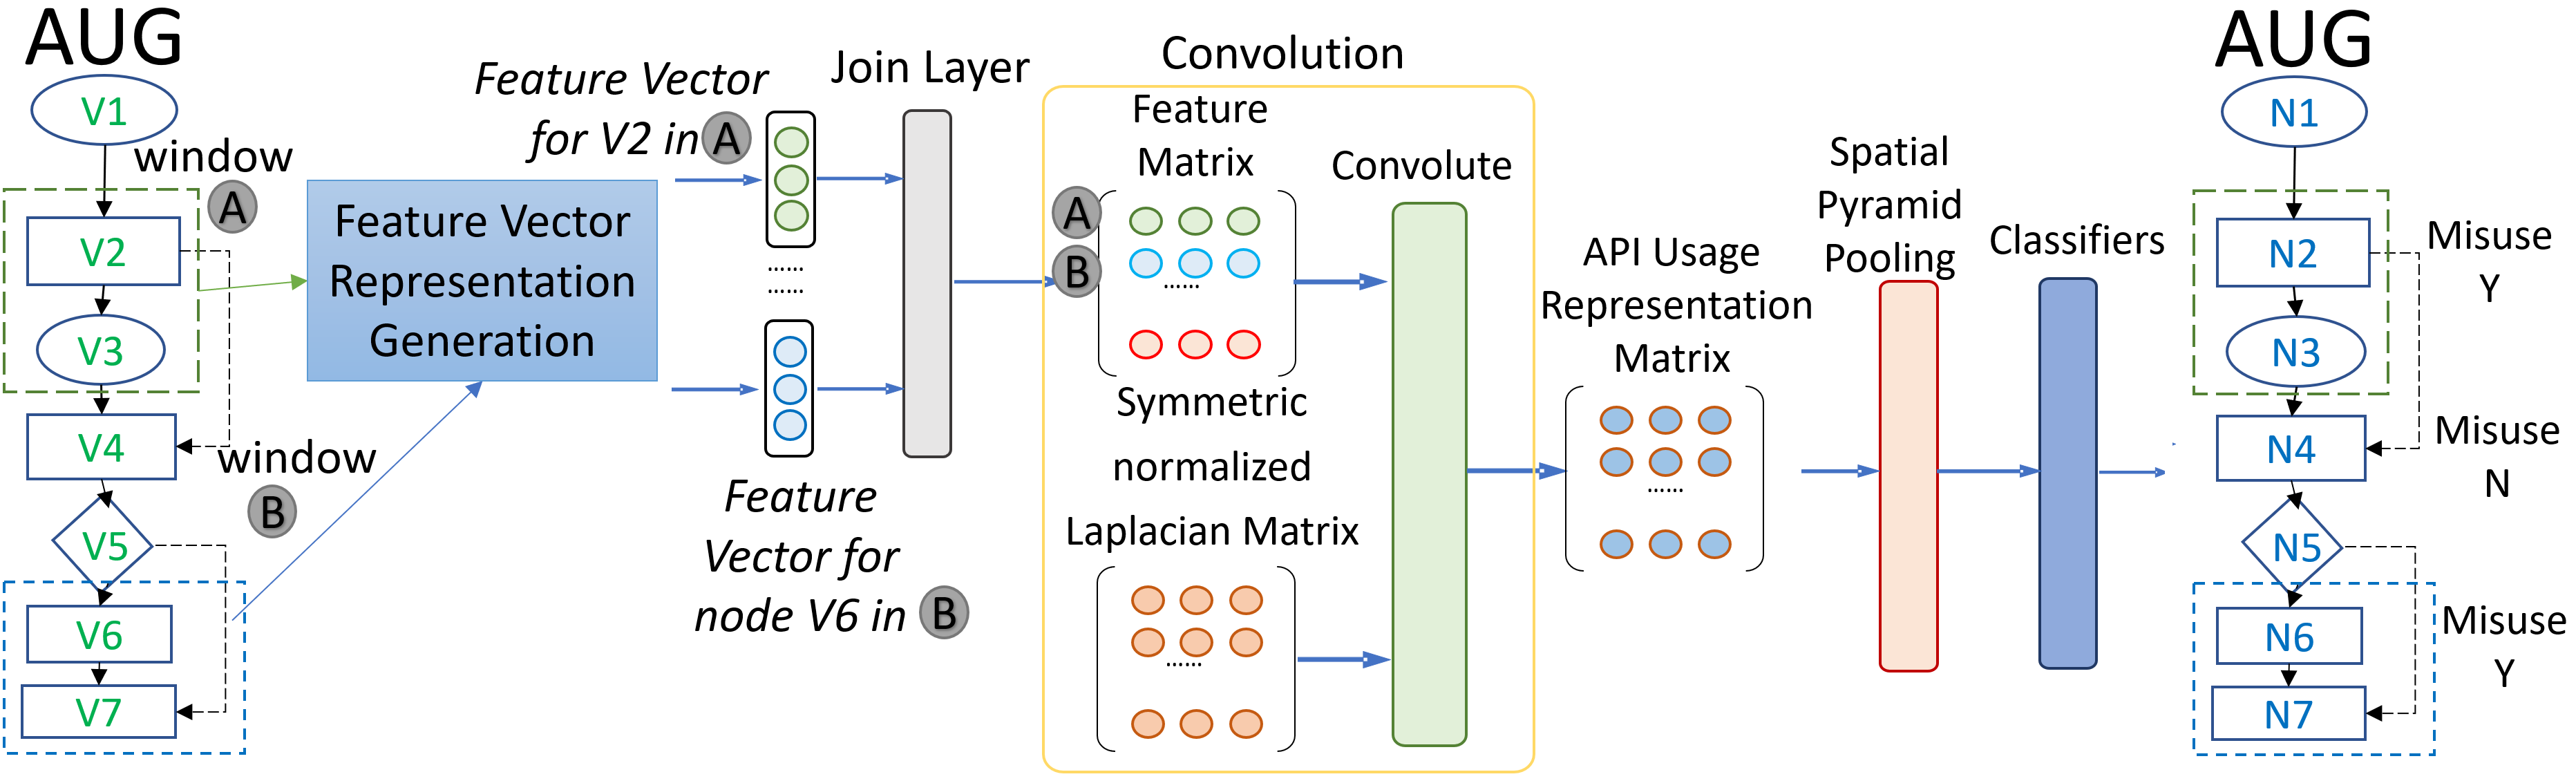
\includegraphics[width=5.8in]{gcn-detection.png}
\vspace{-5pt}
\caption{API Misuse Detection with Label-GCN}
\label{fig:gcn-detection}
\end{center}
\end{figure*}

Fig.~\ref{fig:gcn-detection} presents how we use Labeled, Graph-based,
Convolutional Network (Label-GCN)~\cite{label-gcn} to build the vector
representation (embedding) for an API usage, and then use the learned
vector for API misuse detection. First, we parse a given method $m$
into an API usage graph. Similar to CNN using the filter on an image,
Label-GCN performs sliding a small window along all the nodes of the
AUG. For example, in Figure~\ref{fig:gcn-detection}, the window marked
with \circled{A} for the node $N2$ consists of itself and the
neighboring nodes. Another window (marked with \circled{B}) is for the
node $N6$, including itself and the neighboring nodes. For each
window, Label-GCN generates the feature representation matrix for the
node at the center. For example, for the window centered at $N2$, it
generates the feature vector $F_{N2}$, using the procedure explained in
Section~\ref{sec:features}.

From the representation vectors for all the nodes, Label-GCN uses a
join layer to link all these vectors into the Feature Matrix
$\mathcal{F}_{m}$ for method $m$. A row in the matrix $\mathcal{F}_m$
corresponds to a window in AUG. Next, Label-GCN performs the
convolution operation by first calculating the symmetric normalized
Laplacian matrix~$\tilde{A}$~\cite{GCN16}, and then calculating the
convolution to generate the representation matrix $M_{m}$ for the
method $m$. After that, we use the traditional steps as in a CNN
model: using a spatial pyramid pooling layer (to normalize the method
representation matrix into a uniform size, and reduce its total size),
and connecting its output to a fully connected layer to transform the
matrix into a vector $V_m$ for $m$, which is the
contextualized embedding for the API usage in $m$.





\subsection{API Misuse Detection}

%labeling of each node in the training process: voice 1

With the embedding $V_m$ for the API usage in $m$, we perform
classification by using two hidden layers (controlling the length of
vectors and output) and a softmax function to produce a prediction
result $\mathcal{Y}$ (misuse) or $\mathcal{N}$ (good use) for the API
usage in $m$.

%We use those scores as API misuse scores for the methods in a
%project. The decision for $m$ as $\mathcal{Y}$ or $\mathcal{N}$ for
%API misuse is done via a trainable threshold on the prediction
%score~\cite{li2018vuldeepecker,li2019improving}.

Our model also detects the API misuses at the API element level, i.e.,
the node level in the AUG (Fig.~\ref{fig:gcn-detection}). During
training, the labels for the nodes are handled as follows. If a node
is redundant in an API misuse (i.e., was deleted in a fix), it will be
marked as $\mathcal{Y}$ (misuse). If a node $N$ is inserted for fixing
an API misuse, we will mark any nodes in the old version that have
data and control dependencies with $N$ in the new, fixed version as
$\mathcal{Y}$ (misuse). If a node is modified for fixing, we mark it
as $\mathcal{Y}$ (misuse). Other nodes are marked as
$\mathcal{N}$.
